% !TeX program = pdflatex
% !BIB program = bibtex
% Template LaTeX file for DAFx-19 papers

%------------------------------------------------------------------------------------------
%  !  !  !  !  !  !  !  !  !  !  !  ! user defined variables  !  !  !  !  !  !  !  !  !  !  !  !  !  !
% Please use these commands to define title and author(s) of the paper:
\def\papertitle{On Bad Circuit Modelling}
\def\paperauthorA{Jatin Chowdhury}

% Authors' affiliations have to be set below

%------------------------------------------------------------------------------------------
\documentclass[twoside,a4paper]{article}
\usepackage{dafx_19}
\usepackage{amsmath,amssymb,amsfonts,amsthm}
\usepackage{euscript}
\usepackage[latin1]{inputenc}
\usepackage[T1]{fontenc}
\usepackage{ifpdf}

\usepackage[english]{babel}
\usepackage{caption}
\usepackage{subfig} % or can use subcaption package
\usepackage{xcolor}

\setcounter{page}{1}
\ninept

\usepackage{times}
% Saves a lot of ouptut space in PDF... after conversion with the distiller
% Delete if you cannot get PS fonts working on your system.

% pdf-tex settings: detect automatically if run by latex or pdflatex
\newif\ifpdf
\ifx\pdfoutput\relax
\else
   \ifcase\pdfoutput
      \pdffalse
   \else
      \pdftrue
\fi

\ifpdf % compiling with pdflatex
  \usepackage[pdftex,
    pdftitle={\papertitle},
    pdfauthor={\paperauthorA},
    colorlinks=false, % links are activated as colror boxes instead of color text
    bookmarksnumbered, % use section numbers with bookmarks
    pdfstartview=XYZ % start with zoom=100% instead of full screen; especially useful if working with a big screen :-)
  ]{hyperref}
  \pdfcompresslevel=9
  \usepackage[pdftex]{graphicx}
  \usepackage[figure,table]{hypcap}
\else % compiling with latex
  \usepackage[dvips]{epsfig,graphicx}
  \usepackage[dvips,
    colorlinks=false, % no color links
    bookmarksnumbered, % use section numbers with bookmarks
    pdfstartview=XYZ % start with zoom=100% instead of full screen
  ]{hyperref}
  % hyperrefs are active in the pdf file after conversion
  \usepackage[figure,table]{hypcap}
\fi

% My packages
\usepackage{tikz}
\usetikzlibrary{dsp,chains}
\usepackage{tkz-euclide}
\usetkzobj{all}
\usepackage{cleveref}

\usepackage{listings}
\definecolor{codegreen}{rgb}{0,0.6,0}
\definecolor{codegray}{rgb}{0.5,0.5,0.5}
\definecolor{codepurple}{rgb}{0.58,0,0.82}
\definecolor{backcolour}{rgb}{0.95,0.95,0.92}
 
\lstdefinestyle{mystyle}{
    backgroundcolor=\color{backcolour},   
    commentstyle=\color{codegreen},
    keywordstyle=\color{magenta},
    numberstyle=\tiny\color{codegray},
    stringstyle=\color{codepurple},
    basicstyle=\footnotesize,
    columns=flexible,
    breakatwhitespace=false,         
    breaklines=true,                 
    captionpos=b,                    
    keepspaces=true,                               
    showspaces=false,                
    showstringspaces=false,
    showtabs=false,                  
    tabsize=4
}
 
\lstset{style=mystyle}

\DeclareMathAlphabet{\mathpzc}{OT1}{pzc}{m}{it}
\newcommand{\z}{\mathpzc{z}}

\title{\papertitle}

\affiliation{
\paperauthorA \,}
{\href{http://ccrma.stanford.edu}{Center for Computer Research in Music and Acoustics} \\ Stanford University \\ Palo Alto, CA \\ {\tt \href{mailto:jatin@ccrma.stanford.edu}{jatin@ccrma.stanford.edu}}}

\begin{document}
% more pdf-tex settings:
\ifpdf % used graphic file format for pdflatex
  \DeclareGraphicsExtensions{.png,.jpg,.pdf}
\else  % used graphic file format for latex
  \DeclareGraphicsExtensions{.eps}
\fi

\maketitle
%
\begin{abstract}
Traditional circuit modelling methods typically assume ideal
circuit components. Real world audio circuits exhibit
variations in behavior due to non-ideal factors including
component tolerances, operating temperature, and aging.
We present an brief discussion of each of these non-ideal
factors for resistors, capacitors, and operational amplifiers
(op-amps), and show how they each individually affect the
behavior of a circuit model. We present a model of a Sallen-Key
lowpass filter circuit that incorporates all of the non-ideal factors
together.
\end{abstract}

\section{Introduction} \label{sec:intro}
%
Audio effect circuits and circuit models are a vital part
of modern audio signal processing. Circuit modelling in
particular has seen a risein popularity in recent,
particularly in the form of audio plugin-ins that model
circuits from vintage audio effects, amplifiers, and synthesizers.
Many engineers and musicians prefer these software emulations over
the original hardware units because of the lower cost, portability,
and convenience. However, some users have noticed that the software
emulations do not recreate the unit-to-unit variation in these effects.
For example, if two engineers buy the same hardware compressor unit,
the resulting hardware units will sound similar, but not identical,
due to minor variations in the components that comprise each unit.
Modern circuit models do not attempt to recreate this unit-to-unit
variation, nor do they consider the non-ideal conditions that create
this variation.
\newline\newline
In this writing, we examine these non-ideal conditions, and show how
existing modelling methods can be expanded to include this behavior.
In \S\ref{sec:tol} we examine the effects of component tolerances of resistors
and capacitors. \S\ref{sec:age} discusses the effects of aging capacitors and
resistors. Op-amp aging and temperature considerations are discussed in
\S\ref{sec:op-amp}. Finally, in \S\ref{sec:impl} we show how the above factors
can be implemented into existing circuit models using nodal analysis and
wave digital filters as examples.

\section{Component Tolerances} \label{sec:tol}
%
\begin{figure}[h]
    \center
    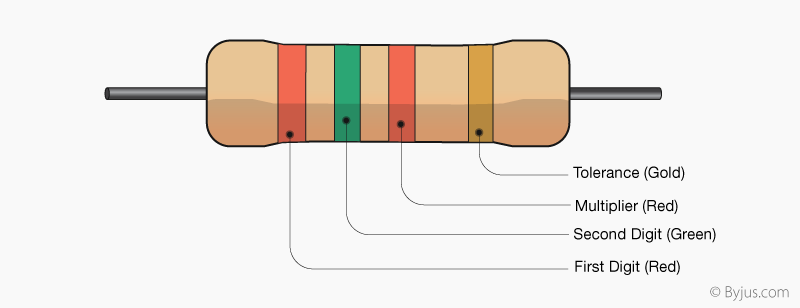
\includegraphics[width=3in]{../CMTolerance/Pics/resistor.png}
    \caption{\label{ResistorLabel}{\it Resistor labelling. Adapted
            from \url{https://byjus.com/physics/resistor-colour-codes/}.}}
\end{figure}
%
\begin{figure}[h]
    \center
    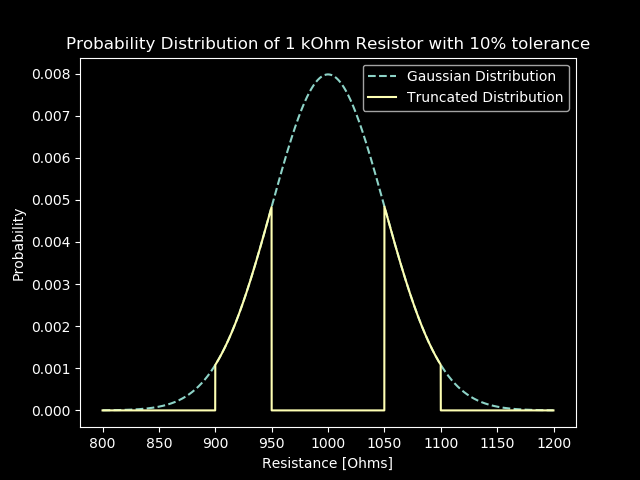
\includegraphics[width=3in]{../CMTolerance/Pics/tgauss_pdf_better.png}
    \caption{\label{trunc_guass}{\it Probability distribution for the
            value of a $10 k\Omega$ resistor with $\pm 10\%$ tolerance.
            Note the ``truncated Gaussian'' distribution.}}
\end{figure}
%
\begin{figure}[h]
    \center
    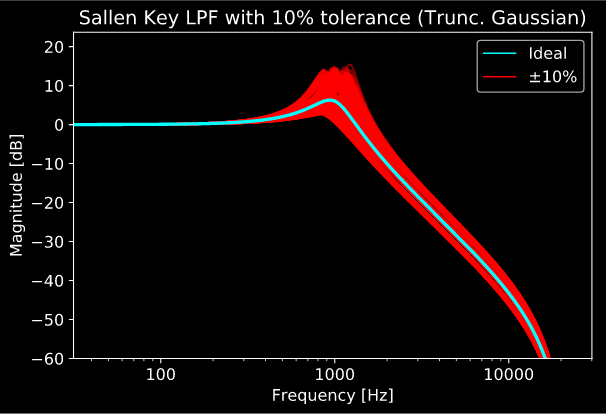
\includegraphics[width=3in]{../CMTolerance/Pics/lpf_tgauss_plot.png}
    \caption{\label{tol_LPF}{\it Frequency response of Sallen-Key lowpass
            filters made with components with $\pm 10\%$ tolerance.}}
\end{figure}
%
All resistors and capacitors are labelled with both a
component value (e.g. $1 k\Omega$ resistor, $1 \mu F$
capacitor), and a tolerance rating (i.e. $\pm 5\%$), as
shown in \cref{ResistorLabel}. We propose adjusting the
component values used in a circuit model to a random
value within the tolerance range of the component.
\newline\newline
When a manufacturer makes a batch of resistors or capacitors
the component values of the batch follows a roughly Gaussian
distribution centered at the ideal component value. The manufacturer
then extracts the worst components that can still satisfy a certain
tolerance rating and sells them at that rating \cite{tolerance}.
For example, if a
manufacturer sells resistors at $\pm 5\%$ and $\pm 10\%$ tolerance
the $\pm 10\%$ components will be distributed in a sort of ``truncated
Gaussian'' distribution, comprised of the original Gaussian
distribution truncated between 5 and 10 \% (see \cref{trunc_guass}).
To show how component tolerances can affect the behavior of an audio
effect circuit, \cref{tol_LPF} shows the frequency response of 1000
Sallen-Key lowpass filters made with components that have $\pm 10\%$
tolerance ratings.
%

\section{Component Aging} \label{sec:age}
%
Stuff\dots

\section{Op-Amp Aging} \label{sec:op-amp}
%
Stuff

\section{Implementation} \label{sec:impl}
%
The structures developed in this study have been implemented as a series of
audio plugins using JUCE/C++. The plugins and their source code are freely
available on GitHub
\footnote{\url{https://github.com/jatinchowdhury18/Bad-Circuit-Modelling}}.

\section{Conclusion} \label{sec:conclusion}
%
In this paper...

\section{Acknowledgments}
%
Ack

%\newpage
% \nocite{*}
\bibliographystyle{IEEEbib}
\bibliography{references}

\end{document}
